\documentclass{article}

\usepackage{fullpage}
\usepackage{color}
\usepackage{amsmath}
\usepackage{url}
\usepackage{verbatim}
\usepackage{graphicx}
\usepackage{mathtools}
\usepackage{parskip}
\usepackage{amssymb}
\usepackage{nicefrac}
\usepackage{listings} % For displaying code
\usepackage{algorithm2e} % pseudo-code
\usepackage{bbm}
% Answers
\def\ans#1{\par\gre{Answer: #1}}
%\def\ans#1{} % Comment this line to produce document with answers

% Colors
\definecolor{blu}{rgb}{0,0,1}
\def\blu#1{{\color{blu}#1}}
\definecolor{gre}{rgb}{0,.5,0}
\def\gre#1{{\color{gre}#1}}
\definecolor{red}{rgb}{1,0,0}
\def\red#1{{\color{red}#1}}
\def\norm#1{\|#1\|}

% Math
\def\R{\mathbb{R}}
\def\argmax{\mathop{\rm arg\,max}}
\def\argmin{\mathop{\rm arg\,min}}
\newcommand{\mat}[1]{\begin{bmatrix}#1\end{bmatrix}}
\newcommand{\alignStar}[1]{\begin{align*}#1\end{align*}}
\def\half{\frac 1 2}
\def\cond{\; | \;}


% LaTeX
\newcommand{\fig}[2]{\includegraphics[width=#1\textwidth]{a4f/#2}}
\newcommand{\centerfig}[2]{\begin{center}\includegraphics[width=#1\textwidth]{a4f/#2}\end{center}}
\newcommand{\matCode}[1]
{\lstinputlisting[language=Matlab]{a4f/#1.m}}
\def\items#1{\begin{itemize}#1\end{itemize}}
\def\enum#1{\begin{enumerate}#1\end{enumerate}}

\let\ask\blu
\let\update\red
\newenvironment{asking}{\begingroup\color{blu}}{\endgroup}
\newcommand\pts[1]{\textcolor{pointscolour}{[#1~points]}}

\begin{document}

\title{CPSC 340 Assignment 4  (\red{due March 13 at 11:55pm)}}
\author{}
\date{}
\maketitle
\vspace{-4em}


\blu{Name(s) and Student ID(s):}

\section{Gaussian RBFs and Regularization}

Unfortunately, in practice we often do not know what basis to use. However, if we have enough data then we can make up for this by using a basis that is flexible enough to model any reasonable function. These may perform poorly if we do not have much data, but can perform almost as well as the optimal basis as the size of the dataset grows. In this question you will explore using Gaussian radial basis functions (Gaussian~RBFs), which have this property. These RBFs depend on a parameter $\sigma$, which (like $p$ in the polynomial basis) can be chosen using a validation set. In this question, you will also see how cross-validation allows you to tune parameters of the model on a larger dataset than a strict training/validation split would allow.

\subsection{Regularization}

If you run the demo \verb|python main.py 1|, it will load a dataset and randomly split the training examples into a ``train" and a ``validation" set (it does this randomly since the data is sorted). It will then search for the best value of $\sigma$ for the RBF basis. Once it has the ``best" value of $\sigma$, it re-trains on the entire dataset and reports the training error on the full training set as well as the error on the test set.

A strange behaviour appears: if you run the script more than once it might choose different values of $\sigma$. Sometimes it chooses a large value of $\sigma$ (like $32$) that follows the general trend but misses the oscillations. Other times it sets $\sigma = 1$ or $\sigma=2$, which fits the oscillations better but overfits so achieves a similar test error.\footnote{This behaviour seems to be dependent on your exact setup. Because the $Z^TZ$ matrix with the RBF matrix is really-badly behaved numerically, different floating-point and matrix-operation implementations will handle this in different ways: in some settings it will actually regularize for you!} \blu{In the file  \texttt{linear\_models.py}, complete the class \texttt{RegularizedRBF}, that fits the model with L2-regularization. Hand in your code, and report the test error you obtain if you train on the full dataset with $\sigma=1$ and $\lambda = 10^{-12}$ (a very small value).}

\pagebreak


\subsection{Cross-Validation}

Even with regularization, the randomization of the training/validation sets has an effect on the value of $\sigma$ that we choose (on some runs it still chooses a large $\sigma$ value).
This variability would be reduced if we had a larger ``train" and ``validation" set, and one way to simulate this is with \emph{cross-validation}. \blu{Modify the training/validation procedure to use 10-fold cross-validation to select $\sigma$ (with $\lambda$ fixed at $10^{-12}$). Hand in your code and report how this affects the selection of $\sigma$ compared to the original code.}


\pagebreak

\subsection{Cost of Non-Parametric Bases}

When dealing with larger datasets, an important issue is the dependence of the computational cost on the number of training examples $n$ and the number of features $d$.

\blu{Answer the following questions and briefly justify your answers:
\enum{
\item What is the cost in big-$\mathcal{O}$ notation of training a linear regression model with Gaussian RBFs on $n$ training examples with $d$ features (for fixed $\sigma$ and $\lambda$)?
\item What is the cost in big-$\mathcal{O}$ notation of classifying $t$ new examples with this model?
\item When is it cheaper to train using Gaussian RBFs than using the original linear basis?
\item When is it cheaper to predict using Gaussian RBFs than using the original linear basis?
}}

\pagebreak

\section{Logistic Regression with Sparse Regularization }

If you run  \verb|python main.py 2|, it will:
\begin{enumerate}
\item Load a binary classification dataset containing a training and a validation set.
\item Standardize the columns of \verb|X|, and add a bias variable (in \verb|utils.load_dataset|).
\item Apply the same transformation to \verb|Xvalidate| (in \verb|utils.load_dataset|).
\item Fit a logistic regression model.
\item Report the number of features selected by the model (number of non-zero regression weights).
\item Report the error on the validation set.
\end{enumerate}
Logistic regression does reasonably well on this dataset,
but it uses all the features (even though only the prime-numbered features are relevant)
and the validation error is above the minimum achievable for this model
(which is 1 percent, if you have enough data and know which features are relevant).
In this question, you will modify this demo to use different forms of regularization
 to improve on these aspects.

Note: your results may vary slightly, depending on your software versions, the exact order you do floating-point operations in, and so on.


\subsection{L2-Regularization }

In \verb|linear_models.py|, you will find a class named \verb|LinearClassifier| that defines the fitting and prediction behaviour of a logistic regression classifier. As with ordinary least squares linear regression, the particular choice of a function object (\verb|fun_obj|) and an optimizer (\verb|optimizer|) will determine the properties of your output model.
Your task is to implement a logistic regression classifier that uses L2-regularization on its weights. Go to \verb|fun_obj.py| and complete the \verb|LogisticRegressionLossL2| class. This class' constructor takes an input parameter $\lambda$, the L2 regularization weight. Specifically, while \verb|LogisticRegressionLoss| computes
\[
f(w) = \sum_{i=1}^n \log(1+\exp(-y_iw^Tx_i)),
\]
your new class \verb|LogisticRegressionLossL2| should compute
\[
f(w) = \sum_{i=1}^n \left[\log(1+\exp(-y_iw^Tx_i))\right] + \frac{\lambda}{2}\norm{w}^2
\]
and its gradient.
\ask{Submit your function object code. Using this new code with $\lambda = 1$, report how the following quantities change: (1) the training (classification) error, (2) the validation (classification) error, (3) the number of features used, and (4) the number of gradient descent iterations.}

Note: as you may have noticed, \verb|lambda| is a special keyword in Python, so we can't use it as a variable name.
Some alternative options:
\verb|lammy|,
\verb|lamda|,
\verb|reg_wt|,
$\lambda$ if you feel like typing it,
the sheep emoji\footnote{Harder to insert in \LaTeX{} than you'd like; turns out there are some drawbacks to using software written in 1978.},
\dots.

\pagebreak

\subsection{L1-Regularization and Regularization Path }
The L1-regularized logistic regression classifier has the following objective function:
\[
f(w) = \sum_{i=1}^n \left[\log(1+\exp(-y_iw^Tx_i))\right] + \lambda\norm{w}_1.
\]
Because the L1 norm isn't differentiable when any elements of $w$ are $0$ -- and that's \emph{exactly what we want to get} -- standard gradient descent isn't going to work well on this objective.
There is, though, a similar approach called \emph{proximal gradient descent} that does work here.%

This is implemented for you in the \verb|GradientDescentLineSearchProxL1| class inside \verb|optimizers.py|.
Note that to use it, you \emph{don't include the L1 penalty in your loss function object};
the optimizer handles that itself.

\begin{asking}Write and submit code to instantiate \verb|LinearClassifier| with the correct function object and optimizer for L1-regularization. Using this linear model, obtain solutions for L1-regularized logistic regression with $\lambda = 0.01$, $\lambda = 0.1$, $\lambda = 1$, $\lambda = 10$. Report the following quantities per each value of $\lambda$: (1) the training error, (2) the validation error, (3) the number of features used, and (4) the number of gradient descent iterations.\end{asking}

\pagebreak

\subsection{L0 Regularization }

The class \verb|LogisticRegressionLossL0| in \verb|fun_obj.py| contains part of the code needed to implement the \emph{forward selection} algorithm,
which approximates the solution with L0-regularization,
\[
f(w) =  \sum_{i=1}^n \left[\log(1+\exp(-y_iw^Tx_i))\right] + \lambda\norm{w}_0.
\]

The class \verb|LinearClassifierForwardSel| in \verb|linear_models.py| will use a loss function object and an optimizer to perform a forward selection to approximate the best feature set.
The \verb|for| loop in its \verb|fit()| method is missing the part where we fit the model using the subset \verb|selected_new|,
then compute the score and updates the \verb|min_loss| and \verb|best_feature|.
Modify the \verb|for| loop in this code so that it fits the model using only
the features \verb|selected_new|, computes the score above using these features,
and updates the variables \verb|min_loss| and \verb|best_feature|,
as well as \verb|self.total_evals|.
\ask{Hand in your updated code. Using this new code with $\lambda=1$,
report the training error, validation error, number of features selected, and total optimization steps.}

Note that the code differs slightly from what we discussed in class,
since we're hard-coding that we include the first (bias) variable.
Also, note that for this particular case using the L0-norm with $\lambda=1$
is using the Akaike Information Criterion (AIC) for variable selection.

Also note that, for numerical reasons, your answers may vary depending on exactly what system and package versions you are using. That is fine.

\pagebreak

\subsection{L2- vs. L1- vs. L0-Regularization}

For this problem, the relevant features are the bias variable and the featurs with prime numbers. Given this, \blu{explain how each of the 3 regularizers (L2-regularization, L1-regularization, and L0-regularization) performed in terms of false positives for feature selection (a false positive would be when a feature is selected but it is not relevant). And then explain how each method did in terms of false negatives.}

\pagebreak


\section{Multi-Class Logistic Regression}

If you run \verb|python main.py 3| the code loads a multi-class
classification dataset with $y_i \in \{0,1,2,3,4\}$ and fits a ``one-vs-all'' classification
model using least squares, then reports the validation error and shows a plot of the data/classifier.
The performance on the validation set is ok, but could be much better.
For example, this classifier never even predicts that examples will be in classes 0 or 4.

\subsection{Softmax Classification}

Linear classifiers make their decisions by finding the class label $c$ maximizing the quantity $w_c^Tx_i$, so we want to train the model to make $w_{y_i}^Tx_i$ larger than $w_{c'}^Tx_i$ for all the classes $c'$ that are not the true label $y_i$.
Here, $c$ is a possible label and $w_{c'}$ is \textbf{row} $c'$ of $W$. Similarly, $y_i$ is the training label and $w_{y_i}$ is \textbf{row} $y_i$ of $W$. Before we move on to implementing the softmax classifier to fix the issues raised in the introduction, let's do a simple example:

Consider the dataset below, which has $30$ training examples, $2$ features, and $3$ class labels:\\
\begin{center}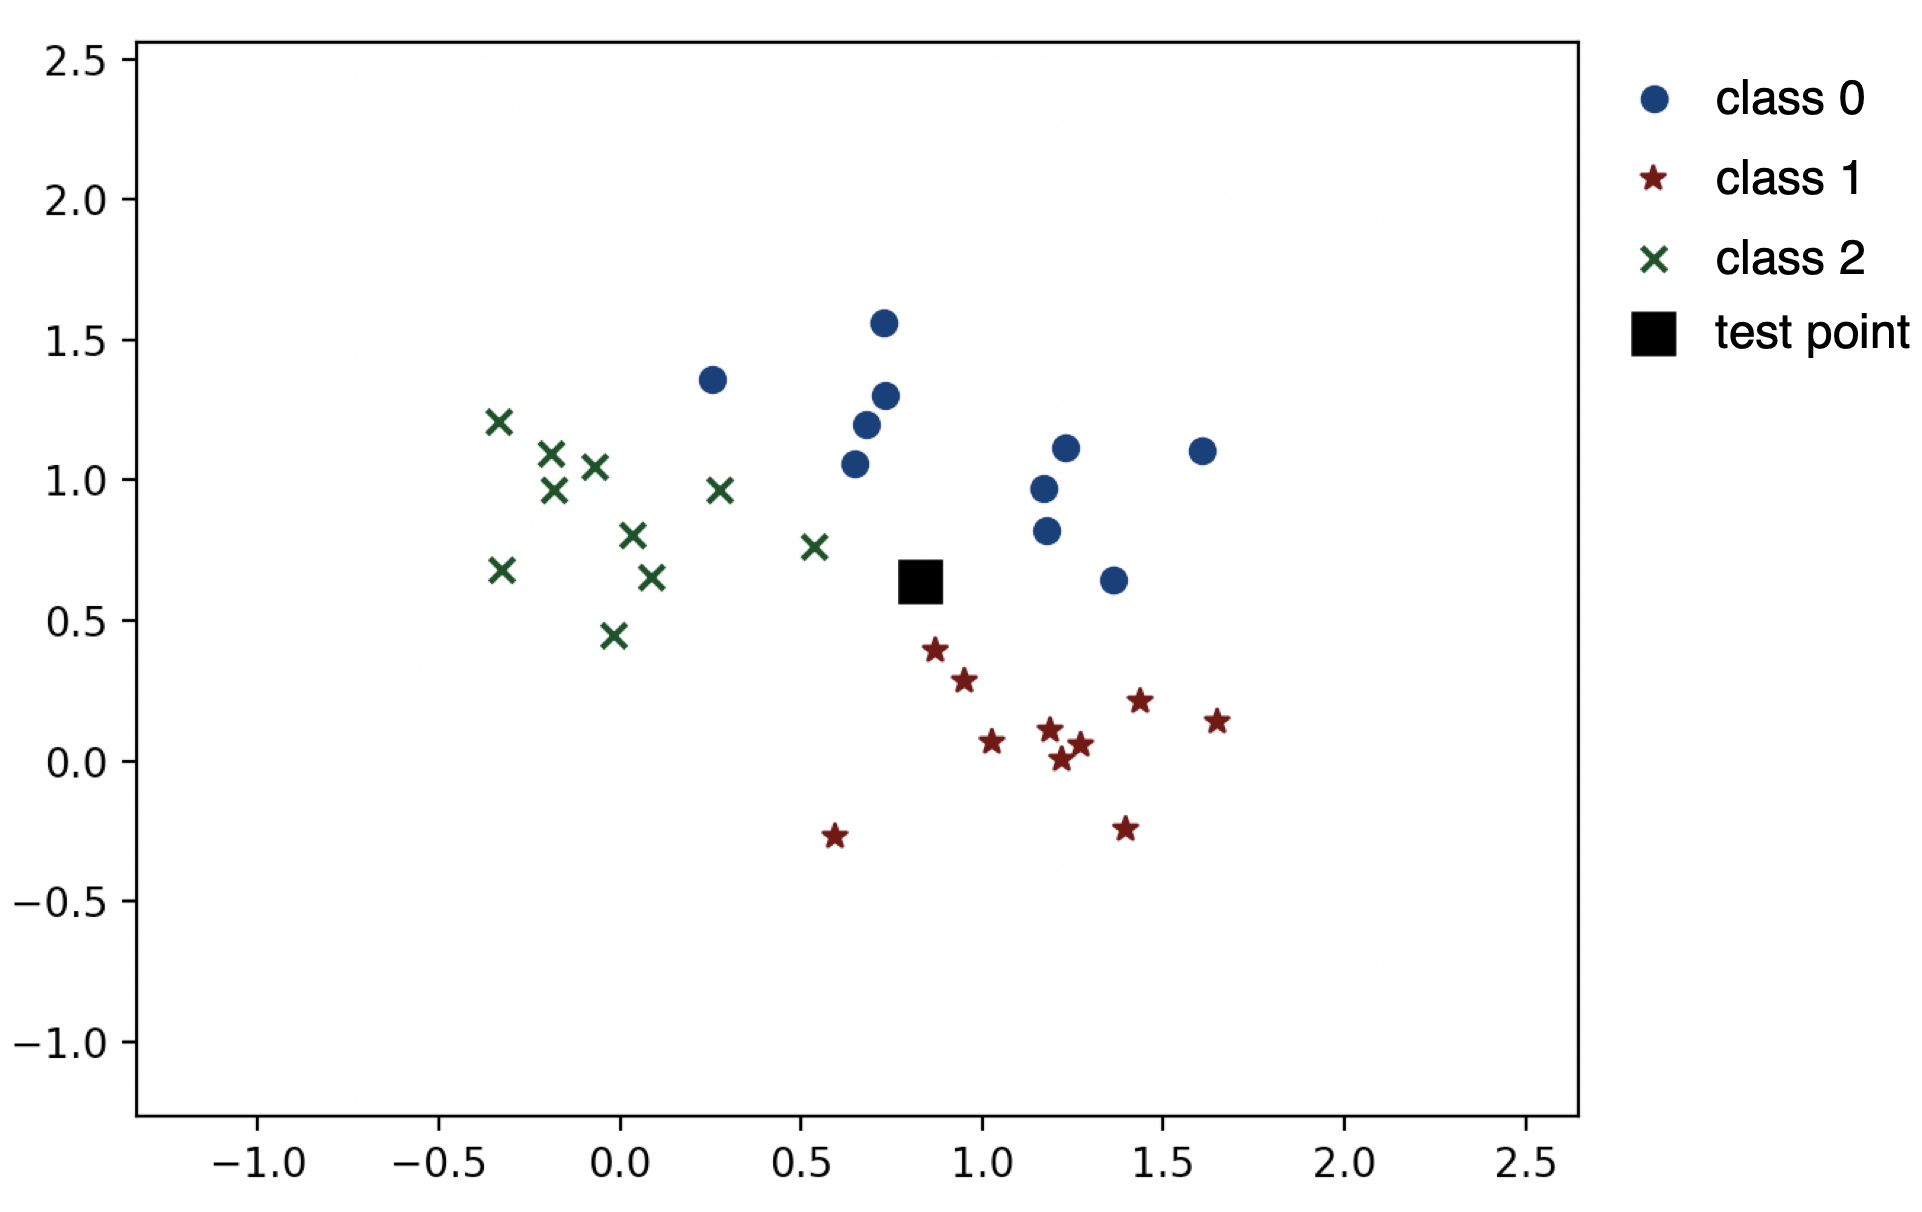
\includegraphics[scale=0.3]{figs/softmaxData.png}\end{center}
Suppose that we want to classify the black square at the location
\[
\hat{x} = \begin{bmatrix}+0.84 \\ +0.64\\ \end{bmatrix}.
\]
Suppose that we fit a multi-class linear classifier including bias variable using the softmax loss. We obtain the weight matrix
\[
\raisebox{-0.28cm}{W =}
\begin{aligned}
            &
            \begin{matrix*}[c]
            \mkern20mu\textrm{bias} & \mkern35mu x^{1} & \mkern25mu x^{2}
            \end{matrix*}
            \\
            &
            \begin{bmatrix*}[r]
                +0.00 & +1.62 & +3.47\\
                +4.90 & -3.83 & +0.67\\
                +3.37 & +2.22 & -4.13 
            \end{bmatrix*},
\end{aligned}
\]
where the first column corresponds to the bias variable and the last two columns correspond to the two features.
\blu{
\begin{enumerate}
\item What is the meaning of the rows $w_i$ in the matrix $W$?
\item Under this model, what class label would we assign to the test example $\hat{x}$? (show your work)
\end{enumerate}}

\pagebreak

\subsection{Softmax Loss}

Using a one-vs-all classifier with a least squares objective hurts performance (1) because the classifiers are fit independently (so there is no attempt to calibrate the \textbf{rows} of the matrix $W$) and (2) because the squared error loss penalizes the model if it classifies examples ``too correctly''. An alternative to this model is to use the softmax loss function, which for $n$ training examples is given by
\[
f(W) = \sum_{i=1}^n \left[-w_{y_i}^Tx_i + \log\left(\sum_{c' = 1}^k \exp(w_{c'}^Tx_i)\right)\right].
\]
\blu{Derive the partial derivative $\frac{\partial f}{\partial W_{cj}}$ of this loss function with respect to a particular element $W_{cj}$ (the variable in row $c$ and column $j$ of the matrix $W$) -- show your work}. Try to simplify the derivative as much as possible (but you can express the result in summation notation).

Hint: for the gradient you can use $x_{ij}$ to refer to element $j$ of example $i$. For the first term you will need to separately think about the cases where $c=y_i$ and the cases where $c\neq y_i$. You may find it helpful to use an `indicator' function, $I(y_i = c)$, which is $1$ when $y_i = c$ and is $0$ otherwise. Note that you can use the definition of the softmax probability to simplify the second term of the derivative.


\pagebreak

\subsection{Softmax Classifier Implementation }

Inside \verb|linear_models.py|, you will find the class \verb|MulticlassLinearClassifier|, which fits $W$ using the softmax loss from the previous section instead of fitting $k$ independent classifiers. As with other linear models, you must implement a function object class in \verb|fun_obj.py|. Find the class named \verb|SoftmaxLoss|. Complete these classes and their methods. \ask{Submit your code and report the validation error.}

Hint: You may want to use \verb|check_correctness()| to check that your implementation of the gradient is correct.

Hint: With softmax classification, our parameters live in a matrix $W$ instead of a vector $w$. However, most optimization routines (like \verb|scipy.optimize.minimize| or our \verb|optimizers.py|) are set up to optimize with respect to a vector of parameters. The standard approach is to ``flatten'' the matrix $W$ into a vector (of length $kd$, in this case) before passing it into the optimizer. On the other hand, it's inconvenient to work with the flattened form everywhere in the code; intuitively, we think of it as a matrix $W$ and our code will be more readable if the data structure reflects our thinking. Thus, the approach we recommend is to reshape the parameters back and forth as needed. The skeleton code of \verb|SoftmaxLoss| already has lines reshaping the input vector $w$ into a $k \times d$ matrix using \verb|np.reshape|. You can then compute the gradient using sane, readable code with the $W$ matrix inside \verb|evaluate()|. You'll end up with a gradient that's also a matrix: one partial derivative per element of $W$. Right at the end of \verb|evaluate()|, you can flatten this gradient matrix into a vector using \verb|g.reshape(-1)|. If you do this, the optimizer will be sending in a vector of parameters to \verb|SoftmaxLoss|, and receiving a gradient vector back out, which is the interface it wants -- and your \verb|SoftmaxLoss| code will be much more readable, too. You may need to do a bit more reshaping elsewhere, but this is the key piece.

Hint: A na\"ive implementation of \verb|SoftmaxLoss.evaluate()| might involve many for-loops, which is fine as long as the function and gradient calculations are correct. However, this method might take a very long time! This speed bottleneck is one of Python's shortcomings, which can be addressed by employing pre-computing and lots of vectorized operations. However, it can be difficult to convert your written solutions of $f$ and $g$ into vectorized forms, so you should prioritize getting the implementation to work correctly first. One reasonable path is to first make a correct function and gradient implementation with lots of loops, then (if you want) pulling bits out of the loops into meaningful variables, and then thinking about how you can compute each of the variables in a vectorized way. Our solution code doesn't contain any loops, but the solution code for previous instances of the course actually did; it's totally okay for this course to not be allergic to Python \verb|for| loops.
\pagebreak

\subsection{Cost of Multinomial Logistic Regression}

Assuming that we have
\items{
\item $n$ training examples.
\item $d$ features.
\item $k$ classes.
\item $t$ testing examples.
\item $T$ iterations of gradient descent for training.
}
\blu{\enum{
\item In big-$\mathcal{O}$ notation, what is the cost of training the softmax classifier (briefly justify your answer)?
\item In big-$\mathcal{O}$ notation, what is the cost of classifying the test examples (briefly justify your answer)?
}}

\pagebreak

\section{Very-Short Answer Questions}

\enum{
\item If we fit a linear regression model and then remove all features whose associated weight is small, why is this an ineffective way of performing feature selection?
\item Given $3$ features $\{f_1, f_2, f_3\}$, provide an argument that illustrates why the forward selection algorithm is not guaranteed to find an optimal subset of features.
\item What is a setting where you would use the L1-loss, and what is a setting where you would use L1-regularization?
\item Among L0-regularization, L1-regularization, and L2-regularization: which yield convex objectives? Which yield unique solutions? Which yield sparse solutions?
\item What is the effect of $\lambda$ in L1-regularization on the sparsity level of the solution? What is the effect of $\lambda$ on the two parts of the fundamental trade-off?
\item Suppose you have a feature selection method that tends not generate false positives but has many false negatives (it misses relevant variables). Describe an ensemble method for feature selection that could improve the performance of this method.
\item How does the hyper-parameter $\sigma$ affect the shape of the Gaussian RBFs bumps? How does it affect the fundamental tradeoff?
\item What is the main problem with using least squares to fit a linear model for binary classification?
\item Suppose a binary classification dataset has 3 features. If this dataset is ``linearly separable'', what does this precisely mean in three-dimensional space?
\item Why do we not minimize $\max(0, -y_i w^\top x_i)$ when we fit a binary linear classifier, even though it’s a convex approximation to the 0-1 loss?
\item For a linearly-separable binary classification problem, how does an SVM classifier differ from a classifier found using the perceptron algorithm?
\item Which of the following methods produce linear classifiers? (a) binary least squares as in Question 3, (b) the perceptron algorithm, (c) SVMs, (d) logistic regression, and (e) KNN with $k=1$ and $n=2$.
\item Why do we use the polynomial kernel to implement the polynomial basis when $d$ and $p$ (degree of polynomial) are large?
\item What is the relationship between the softmax loss and the softmax function?
}

\end{document}